
% this file is called up by thesis.tex
% content in this file will be fed into the main document

%: ----------------------- introduction file header -----------------------
\chapter{Creation and Publication of Probabilistic Topic Models}\label{ch:scalability}

\graphicspath{{scalability/figures/}}

% -------------------------------------------------------------
% -- Scalability
% -------------------------------------------------------------

This chapter present \textit{\textbf{librAIry}} \citep{Badenes-Olmedo2017}, our framework to create, publish and exploit probabilistic topic models through a service-oriented approach. In doing so, we reuse existing techniques and standards, which aim to make our results reusable and interoperable with other alternative approaches.


\section{Distributed Topic Modeling}


There are numerous and varied domains where probabilistic topic models have been successfully used in recent years \citep{TapiNzali2017, ONeill2017, Greene2016, He2017}. Each one of them with its particularities. Some with only a few documents, and others with thousands, and even millions, texts. There are environments with only one processor, or environments with multiple processors spread over one or several distributed machines. Taking into account such diversity, topic modeling algorithms have evolved to improve their efficiency in challenging situations, but they only cover the training process of the model. The probabilistic topic model life-cycle begins with text pre-processing, continues with model training, follows with model distribution, and ends with model exploitation. In order to have a framework that covers the entire process of creating probabilistic topic models in both large- and small-scale, we have focused on adapting and reusing techniques and standards widely used in software engineering domain. 

\textit{librAIry} is a framework to manage probabilistic topic models that combines training algorithms with natural language processing tools to create and distribute models suitable for stand-alone use. The main objective is to facilitate the creation of reusable topic models by minimizing their technical dependencies. Methods and algorithms proposed in this thesis have been implemented and evaluated in this framework, which therefore serves as the technological basis for our research.

Our design requirements, which have guided our development process, can be organized into three categories:
\begin{itemize}
\item \textbf{Corpora representation requirements}, which tackle the modeling of document collections and its metadata. This includes texts and their related annotations.
\item \textbf{Task distribution requirements}, which refer to event management to notify changes in document collections. Coordination of this information is crucial for robust and reproducible results.  
\item \textbf{Process execution requirements}, which capture the operations involved in creating a topic model. The parallel task execution leads to the creation of models.
\end{itemize}

The rest of the section describes how we have adapted existing techniques and standards in \textit{librAIry} to address each of the requirements categories described above. An open, distributed and scalable framework has been developed whose source code is publicly available for reuse\footnote{\url{https://github.com/librairy}}.

\subsection{Representing Corpora for Topic Modeling}

Inspired by a Staged Event-Driven Architecture (SEDA) that exchanges messages and handle status changes, our framework is based on \textit{resources} and \textit{actions}. A \textit{resource} can be a \textit{document} that represents raw texts (e.g. a full-text research paper), or a \textit{snippet} of text with a logical part  (e.g. sections, summaries or even phrases grouped by their rhetoric), or a \textit{domain} that contains a dataset of texts (e.g. a conference proceedings) or even an \textit{annotation} made on them (e.g. review comments, named-entities, topics). \textit{Actions} can be executed on these resources (e.g. \textit{create}, \textit{update} or \textit{delete}), to change their status (e.g. \textit{created}, \textit{updated} or \textit{deleted}).

To better illustrate this model, take the research articles published at the latest K-CAP conference\footnote{\url{http://www.k-cap.org/2019}} (See fig. \ref{fig:librairy-model}). A new \textit{document} is created for each publication with the full text of the article. Each \textit{document} is then associated with several \textit{snippets}, one for each section of the article. Finally, a \textit{domain} is created that groups all these \textit{documents} under the same conference. This initial representation can be extended with \textit{annotations}, that can provide more detailed information at different levels (e.g. named-entities, topics, or keywords).

% 
\begin{figure}
  \center
  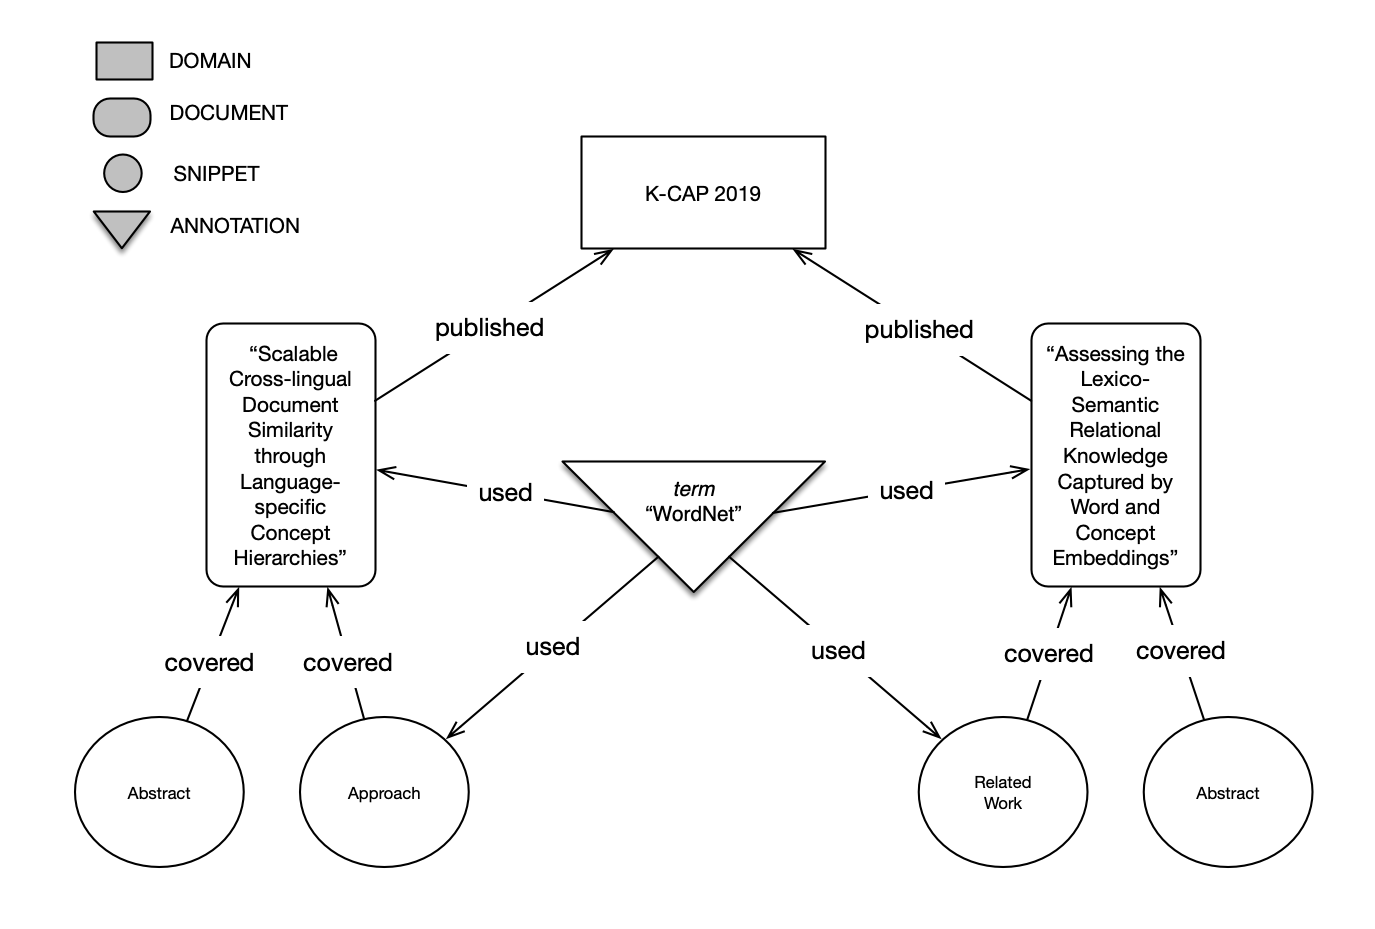
\includegraphics[scale=0.55]{model}
  \caption{Representation of two scientific papers published at the International Conference on Knowledge Capture (K-CAP, 2019) that mention the same entity, Wordnet, in different sections.}
  \label{fig:librairy-model}
\end{figure}
% -----------

\textit{Resources}, \textit{actions} and \textit{states} are individually addressable and linkable \citep{Turchi2012a} following the Linked Data principles\citep{Bizer2009}. Each of them has: (1) a name, (2) a retrievable (or dereferenceable) HTTP URI so that it can be looked up, (3) a descriptive information provided by using standard notation (e.g. JavaScript Object Notation (JSON)) when it is  looked up by URI, and (4) links to other URIs so that other resources can be discovered from it.

More details about each of them is shown below.

\subsubsection{Domain}

A \textit{domain} is an aggregation of \textit{documents}. It is described as a group with parts separately described. A default \textit{domain} is created and every \textit{document} belongs, at least, to one \textit{domain} (Fig \ref{fig:librairy-model-domain}).

A \textit{domain} can contain the following information: 
\begin{itemize}
\item \textbf{uri}: identifier created from the resource type (i.e \textit{domains}) and a Universally Unique Identifer (UUID) (e.g \textit{domains/88b86fa6-11c8-11eb-adc1-0242ac120002})
\item \textbf{creation-time}: date when resource was created. It follows the ISO-8601\footnote{\url{https://www.iso.org/standard/40874.html}}.
\item \textbf{name}: label associated to the resource.
\item \textbf{description}: additional information about it.
\end{itemize}

\begin{figure}
  \center
  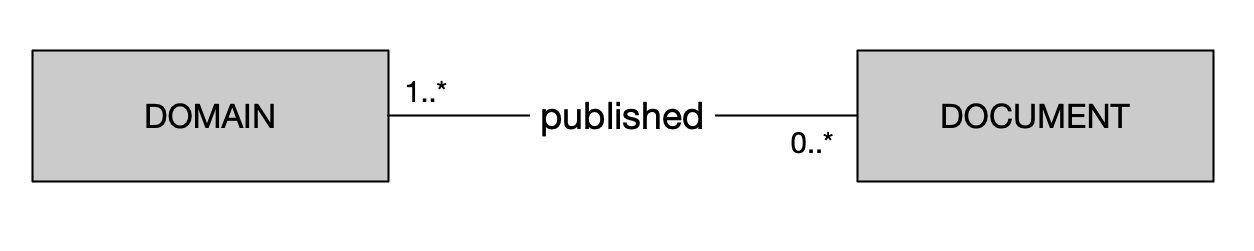
\includegraphics[scale=0.45]{model-domain.png}
  \caption{Relation between \textit{domain} and \textit{document}.}
  \label{fig:librairy-model-domain}
\end{figure}

\subsubsection{Document}

A \textit{document} is a resource consisting primarily of words for reading. Examples include research papers, articles, books or patents. It follows the Open Archives Initiative for Object Reuse and Exchange\footnote{\url{http://www.openarchives.org}} (OAI-ORE) and the Dublin Core Metadata Initiative\footnote{\url{http://dublincore.org}}. 

A \textit{document} can contain the following information:                                                              

\begin{itemize}
\item \textbf{uri}: identifier created from the resource type (i.e \textit{documents}) and a UUID ( e.g \textit{documents/809af686-11c8-11eb-adc1-0242ac120002})
\item \textbf{creation-time}: date when resource was created. It follows the ISO-8601.
\item \textbf{publishedOn}: date when resource was published. It follows the ISO-8601.
\item \textbf{publishedBy}: an entity responsible for making the document available. It can be a  person, an  organization or a service. It may be different from the entity that conceptually formed the resource (e.g. wrote the document), which is recorded as \textit{authoredBy}. This entity should be identified by a valid Uniform Resource  Identificator (URI) such as WebId\footnote{\url{http://www.w3.org/wiki/WebID}}, orcid\footnote{\url{http://orcid.org}} or internal URI. 
\item \textbf{authoredOn}: the time the \textit{document} was conceptually formed. The author time should be present if different from \textit{publishedOn}. It must be a formatted timestamp following ISO-8601.
\item \textbf{authoredBy}: an entity primarily responsible for making the content of the \textit{document}. It may be a list to indicate multiple authors. Each of them identified by a valid URI such as WebId, orcid or internal URI.
\item \textbf{retrievedFrom}: a URI identifying the repository or source from which the document was derived. This property should be accompanied with \textit{retrievedOn}.
\item \textbf{retrievedOn}: the time the \textit{document} was retrieved on. If this property is present, the \textit{retrievedFrom} must also be present. It must be a formatted timestamp following ISO-8601.
\item \textbf{format}: the physical or digital manifestation of the resource. Typically, it includes the media-type (i.e the IANA code\footnote{\url{http://www.iana.org}}) of the \textit{document}.
\item \textbf{language}: the language(s) in which the document was written. It is defined by RFC-1766\footnote{\url{http://www.ietf.org/rfc/rfc1766.txt}} with a two-letter language code followed, optionally, by a two-letter country code.
\item \textbf{title}: a name given to the \textit{document}. It is a name by which the \textit{document} is formally known.
\item \textbf{description}: it may include but is not limited to an abstract, or a free-text account of the content.
\item \textbf{rights}: information about rights helds in and over the \textit{document}.
\item \textbf{content}: raw text from the \textit{document}.
\end{itemize}

Furthermore, a \textit{document} can contain zero or more \textit{snippets} and a \textit{snippet} can belong to one or more \textit{documents}. Since \textit{librAIry} can also discover analogies among \textit{documents}, a \textit{document} may contain zero or more references to other \textit{documents} (Fig. \ref{fig:librairy-model-document}).

\begin{figure}
  \center
  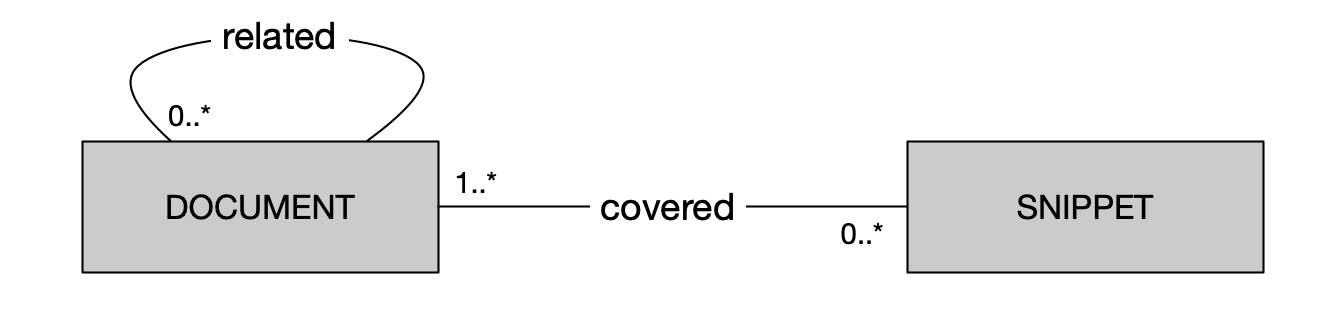
\includegraphics[scale=0.45]{model-document.png}
  \caption{Relation between \textit{document} and \textit{snippet}.}
  \label{fig:librairy-model-document}
\end{figure}

\subsubsection{Snippet}

A \textit{snippet} is a resource that is included either physically or logically in a \textit{document}. In a scientific \textit{document}, for example, it may be the \textit{abstract} section or a logical set of sentences sharing the same rhethorical class (e.g. approach, background, related-work, etc). As seen above (Fig. \ref{fig:librairy-model-document}), a \textit{snippet} can belong to one or more \textit{documents}.

It contains the following information:
\begin{itemize}
\item \textbf{uri}: identifier created from the resource type (i.e \textit{snippets}) and a UUID ( e.g \textit{snippets/7a5a46c8-11c8-11eb-adc1-0242ac120002})
\item \textbf{creation-time}: date when resource was created. It follows the ISO-8601\footnote{\url{https://www.iso.org/standard/40874.html}}.
\item \textbf{sense}: content-type. It refers to a section or any other criteria under which the following text makes sense.
\item \textbf{content}: partial text retrieved from the full-text of the \textit{document}.
\end{itemize}

\subsubsection{Annotation}

\textit{Annotations} are data retrieved from resources that can be used to relate them. They are basically key-value data structures associated to \textit{domains}, \textit{documents} or \textit{snippets}. Examples are entities mentioned in a text, or topics covered in a collection. Any resource can have zero or multiple annotations, which can be shared among several resources (Fig. \ref{fig:librairy-model-annotation})

It contains the following information:
\begin{itemize}
\item \textbf{uri}: identifier created from the resource type (i.e \textit{annotations}) and a UUID ( e.g \textit{annotations/73671e68-11c8-11eb-adc1-0242ac120002})
\item \textbf{creation-time}: date when resource was created. It follows the ISO-8601\footnote{\url{https://www.iso.org/standard/40874.html}}.
\item \textbf{key}: a category or type associated with the information it contains (e.g. entity, comment, topic, keywords, etc). Recommended best practice is to use a controlled vocabulary.
\item \textbf{value}: a note about the resource in the form of free text..
\end{itemize}

\begin{figure}
  \center
  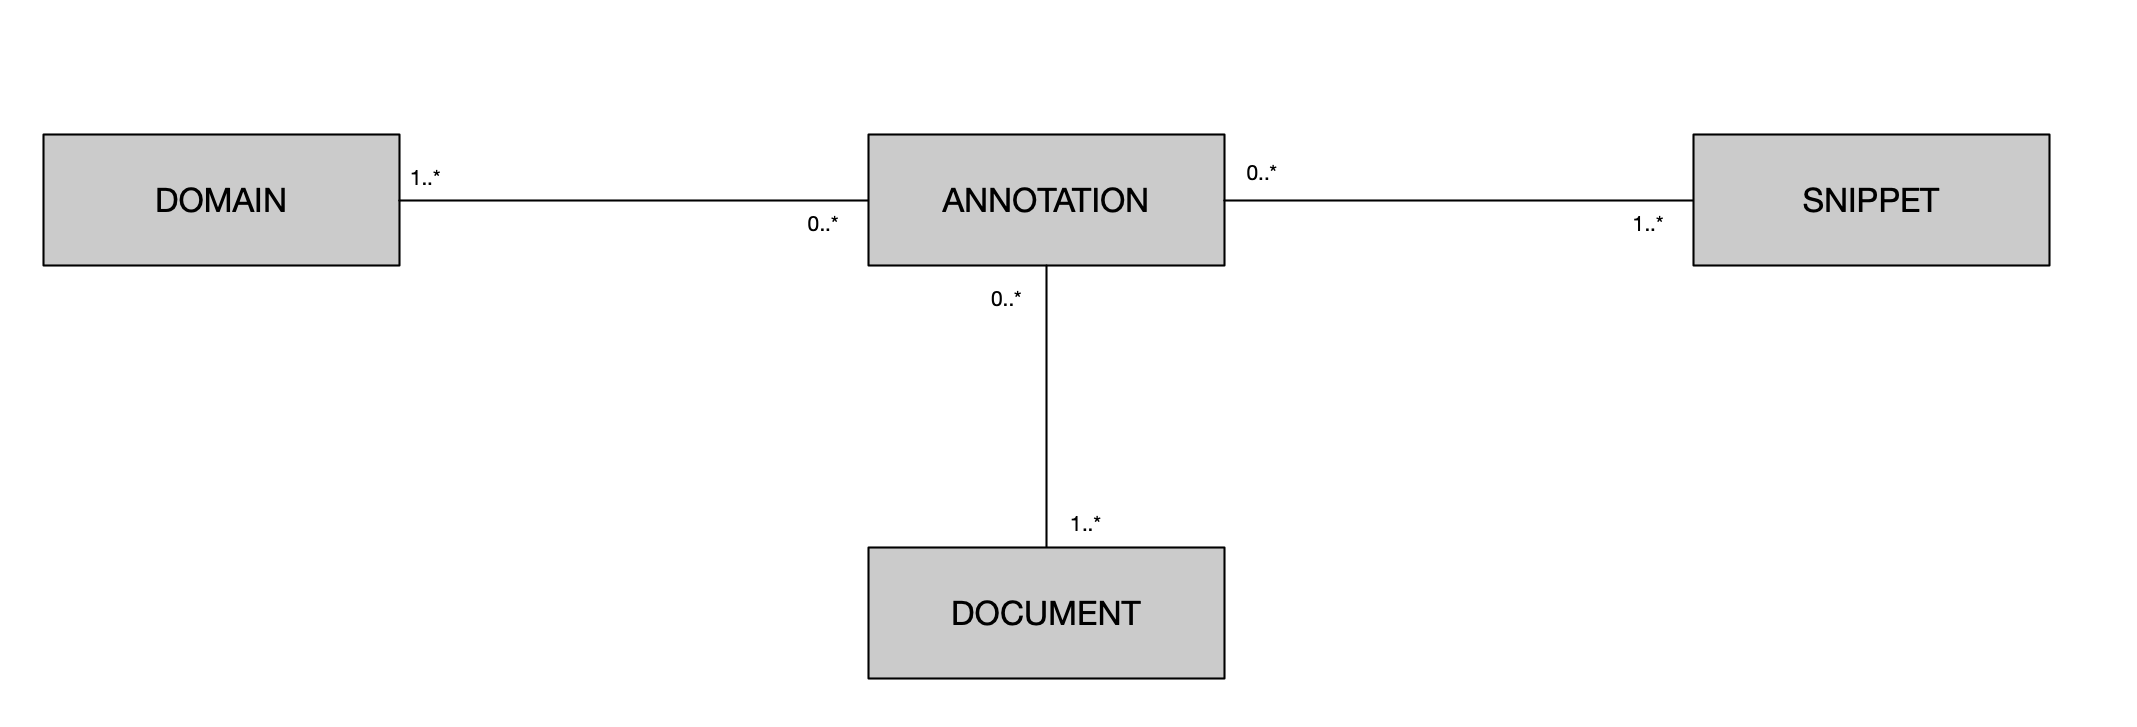
\includegraphics[scale=0.4]{model-annotation.png}
  \caption{Relation between \textit{annotations} and other resources.}
  \label{fig:librairy-model-annotation}
\end{figure}

\subsection{Event-oriented Processing Workflow}

Along with the resources mentioned above, there are two additional elements that provide a special behavior to the system: \textit{modules} and \textit{events}. An \textit{event} is a non-persistent time-based occurrence that describes a new action performed on a resource. \textit{Modules} are responsible for carrying out operations on the resources (e.g. tokenize a \textit{document} or create a topic model from a \textit{domain}). \textit{Events} are broadcasted so that any \textit{module} is aware of the changes made to the resources and  can perform actions on one or more resources in response to a new state reached by a given resource. These actions are paralleled since modules are replicated through distributed environments.

\begin{figure}
  \center
  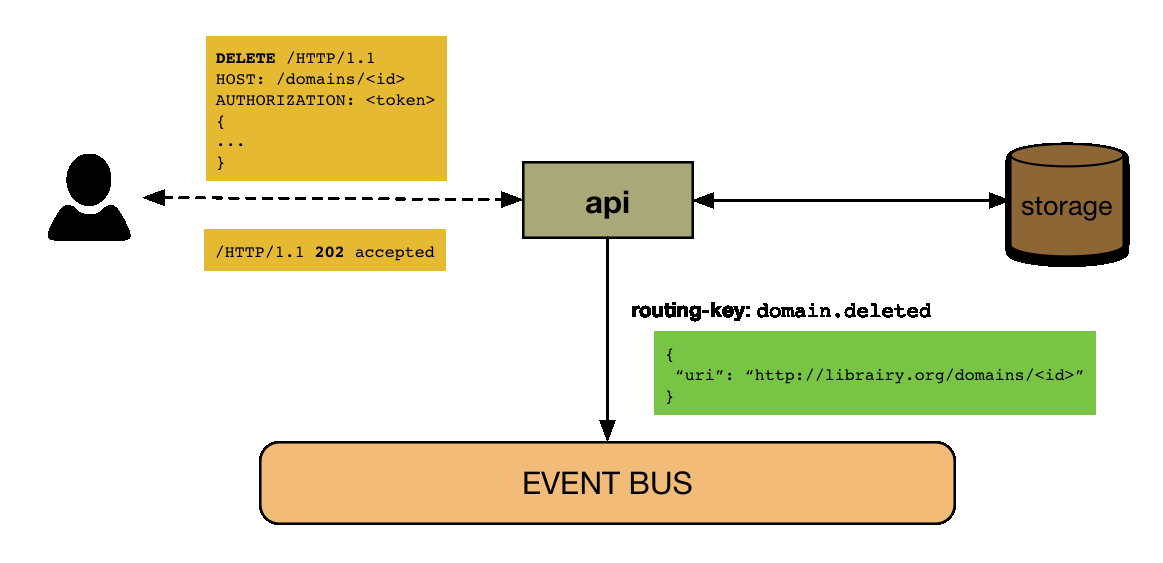
\includegraphics[scale=0.45]{api-domain-deleted}
  \caption{Domain deleted flow.}
  \label{fig:librairy-domain-deleted}
\end{figure}


The framework follows a publisher/subscriber approach where \textit{modules} can publish and read \textit{events} to notify and to be notified about the state of a \textit{resource} (Fig. \ref{fig:librairy-states}). An \textit{event} notifies a performed action (i.e. a resource and its new state), and follows the Representational State Transfer (REST)\cite{Fielding2002} paradigm. It contains the resource type and the new state reached by a specific resource ( i.e \textit{created}, \textit{deleted} or \textit{updated}). For example, when a new \textit{domain} is created, an \textit{event} message is published to the channel: $domain.created$. A channel is a space where \textit{events} are published and \textit{modules} can be subscribed to read only some \textit{events}. The actions performed by a module depend on the events to which it is subscribed. Therefore, the workflow of the framework is neither static nor explicitly defined. A distributed workflow emerges according to the \textit{modules} subscribed to the \textit{event} channels.

We used the Advanced Message Queuing Protocol (AMQP) as the messaging standard to avoid any cross-platform problem and any dependency to the selected message broker (i.e the server that sends and receives messages). This protocol defines: \textit{exchanges}, \textit{queues}, \textit{routing-keys} and \textit{binding-keys} to communicate publishers (i.e message senders) and consumers (i.e message readers). \textit{Exchanges} are like message inboxes, and \textit{queues} are subscribed to them by specifying the message types they are interested in with a \textit{binding-key}. A message sent by a publisher to an exchange is routed with a \textit{routing-key} and consumers matching that \textit{routing-key} with their \textit{binding-key} (used to connect the \textit{queue} to that \textit{exchange}), will receive the message. This mechanism allows sending and receiving messages between consumers and producers by means of shared keys (i.e. \textit{routing-keys} and \textit{binding-keys}). A key follows the structure: \textit{resource.status}. Since a wildcard-based definition can be used to set the key, this paradigm allow modules both listening to individual type events (e.g. \textit{domains.created} for new \textit{domains}), or multiple type events (e.g. \textit{\#.created} for all new resources).


\begin{figure}
  \center
  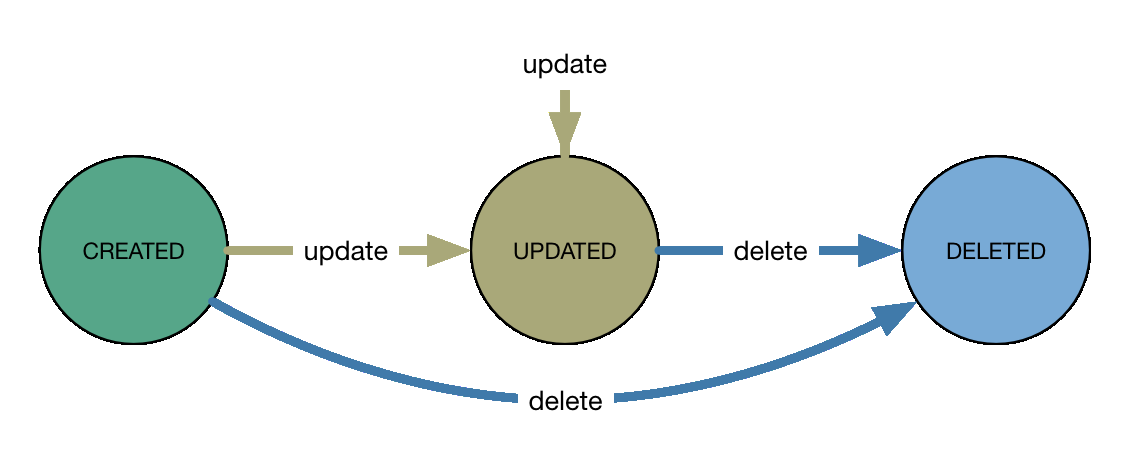
\includegraphics[scale=0.3]{resource-states}
  \caption{Resource states.}
  \label{fig:librairy-states}
\end{figure}


\subsection{Combined Modular Execution}

A microservice-oriented style has been used to define the framework architecture. Through multiple services the system analyzes texts, creates probabilistic topic models, publishes them as new services and uses them to annotate texts. A service is equivalent to a functionality, and each functionality is materialized by a module in the system. A module is then a cohesive and independent process \cite{Dragoni2016} with a specific purpose (i.e functionality) based on the events to which it responds. These events correspond to the routing- and binding- keys attached to the module.

There are four types of modules (Fig. \ref{fig:librairy-modules}):
\begin{itemize}
	\item \textbf{Harvester}: creates resources such as \textit{documents}, \textit{snippets} and \textit{domains}, from local or remote repositories with textual files.
    \begin{itemize}[rightmargin=\dimexpr\linewidth-5cm-\leftmargin\relax]
    		\item \textit{binding-queue} (i.e listening for): nothing
		\item \textit{routing-key} (i.e publishing to): \textit{document.created}, \textit{snippet.created}, \textit{domain.(created;updated)}
    \end{itemize}
    \item \textbf{Annotator}: makes NLP annotations (i.e named-entities, bag-of-words, etc) and infers topics in \textit{documents} and \textit{snippets}. 
    \begin{itemize}[rightmargin=\dimexpr\linewidth-5cm-\leftmargin\relax]
    	\item \textit{binding-key}: \textit{document.(created;updated)}, \textit{snippet.(created;updated)}
		\item \textit{routing-key}: \textit{annotation.(created;deleted)}
    \end{itemize}
    \item \textbf{Modeler}: creates a probabilistic topic model from a given \textit{domain}. It uses the texts of its \textit{documents} to train a topic model.
    \begin{itemize}[rightmargin=\dimexpr\linewidth-5cm-\leftmargin\relax]
    	\item \textit{binding-key}: \textit{domain.(created;updated)}
		\item \textit{routing-key}: \textit{annotation.(created;deleted)}	
	\end{itemize}
	\item \textbf{Administrator}: performs user-driven tasks such as reading/writing resources or database queries.	
    \begin{itemize}[rightmargin=\dimexpr\linewidth-5cm-\leftmargin\relax]
    	\item \textit{binding-key}: nothing
		\item \textit{routing-key}: \textit{domain.(created;updated;deleted)}, \textit{document.(created;updated;deleted)}, \textit{snippet.(created;updated;deleted)}, and \textit{annotation.(created;updated;deleted)}
    \end{itemize}
\end{itemize}

\begin{figure} 
  \center
  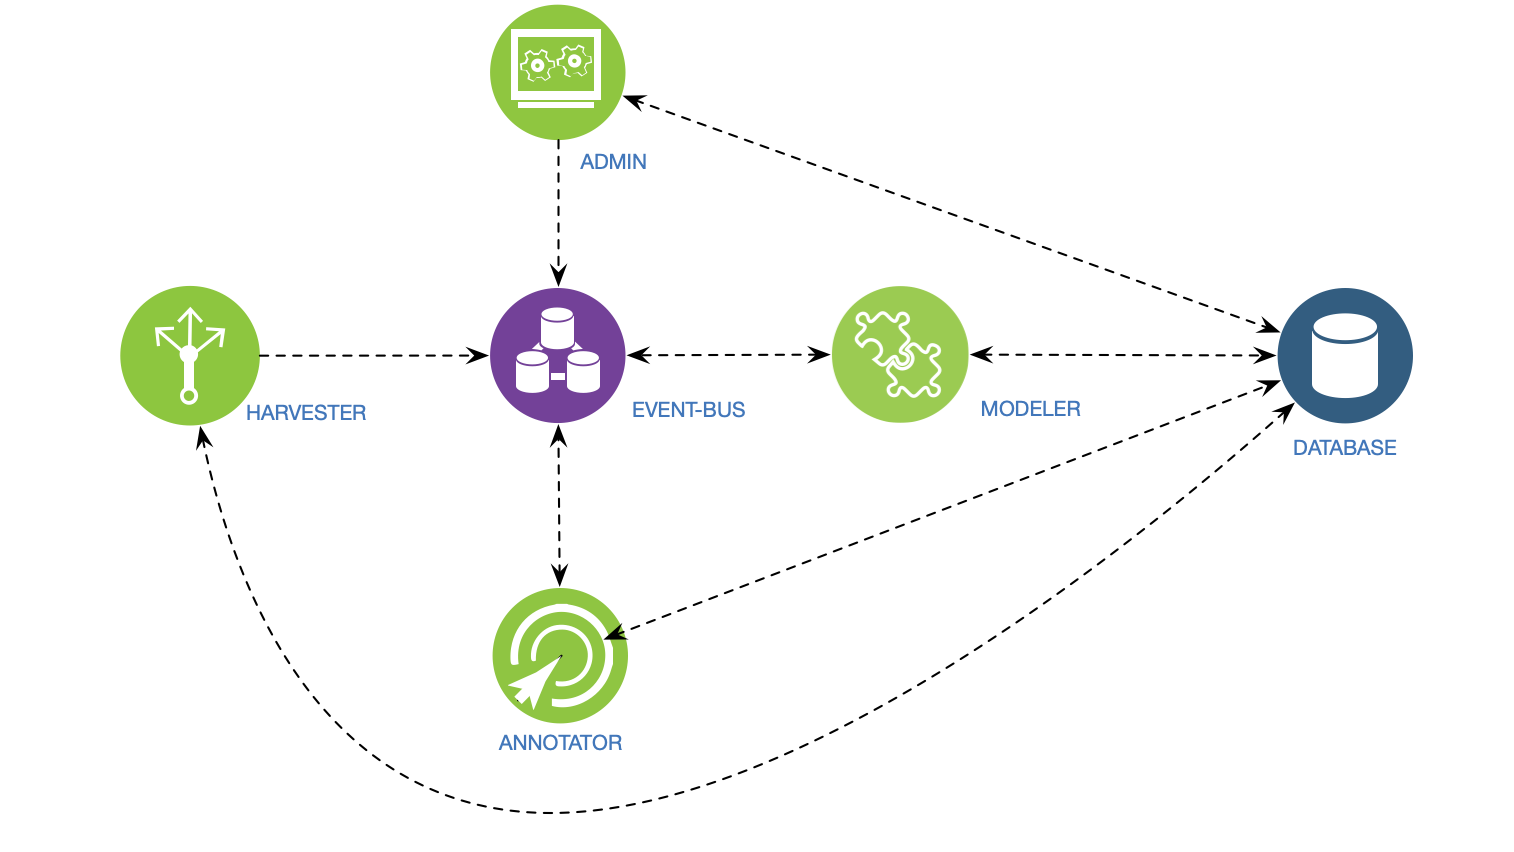
\includegraphics[scale=0.45]{modules}
  \caption{Modules.}
  \label{fig:librairy-modules}
\end{figure}


Each module is wrapped with an Application Program Interface (API) over HTTP, that follows the web standards for the RESTful API development, and a Avro\footnote{\url{https://avro.apache.org}}-based interface over TCP for efficiency reasons. Figure 4 shows a sequence diagram that illustrates how modules work to create a topic model when new documents are added to the framework. 

\begin{figure} 
  \center
  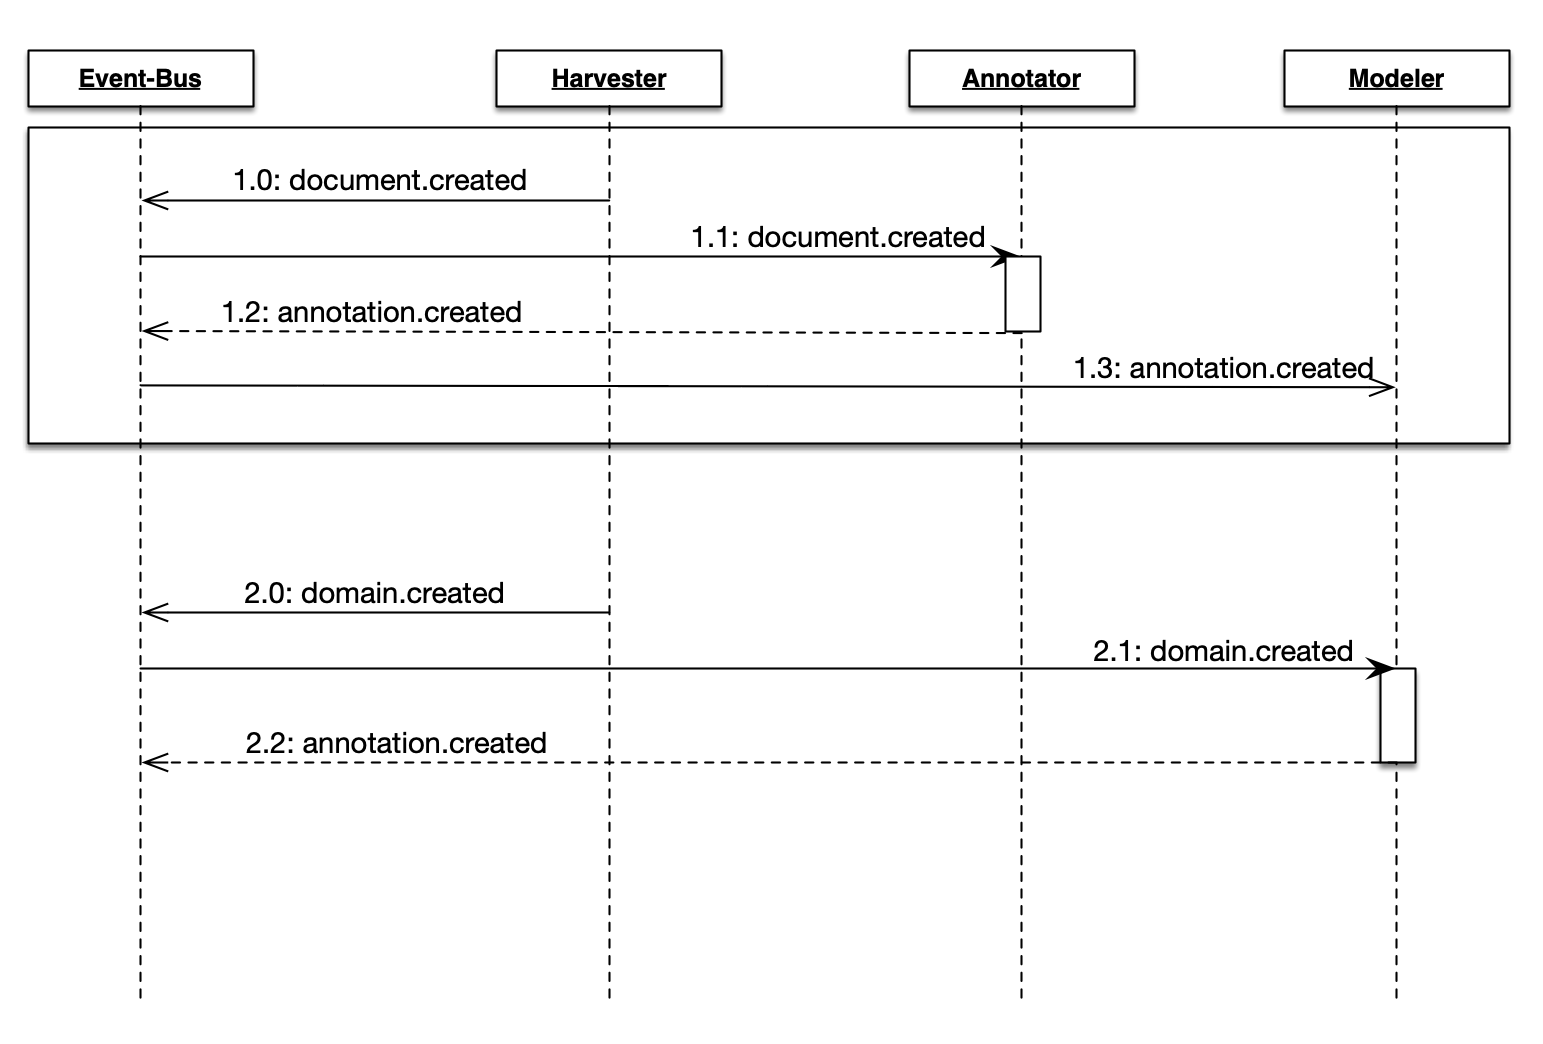
\includegraphics[scale=0.45]{librairy-sequence.png}
  \caption{Sequence of messages exchanged between modules to create a topic model from the documents added to a domain.}
  \label{fig:librairy-modules}
\end{figure}




\section{Reusable Topic Modeling}



% existentes herramientas de análisis de textos: escalabilidad vertical

% en que consiste los modelos probabilísticos de tópicos para necesitar tareas de NLP


%In natural language processing, the term topic means a set of words. These are the words that come to mind when thinking of this topic. For example music could associate the words sound, instrument and composition. Without going more deep now, a topic model automatically discovers the words that are most likely to describe the topics present in a document collection. A trained model may then be used to infer which of these topics occur in new documents and can also pick out which portions of a document cover which topics.

%The learning process in a topic model first requires creating bag-of-words (BoW) from texts. A BoW contains the frequencies of each word in a text. The model uses these representations to discover the word distributions that best define the topics to fit their presences in the documents, assuming that a document can covers several topics. Take the following text: "Apple has just released in its Apple Store a video celebrating International Women's Day, about the lives of several relevant women, especially the most influential young woman in recent years.". A basic approach would transform that text into a BoW that considers whitespaces and punctuation marks as word separators (e.g. 'Apple'(2), 'has'(1), 'just'(1), etc). But this approach makes several mistakes. 'Apple' does not appear twice, but only once, as 'Apple Store' is different to 'Apple'. Some natural language processing tasks are needed to make these assessments. Using Named Entity Recognition (NER) techniques, for example,  'Apple', 'Apple Store' and 'International Women's Day' are different words in a BoW. Sometimes a normalization is applied to group plural and singular nouns. Using stemming techniques and Part-of-Speech (PoS) tagging, 'women' and 'woman' are transformed into a same word, 'woman', with a frequency equals to the sum of their frequencies, in this case 2. This is just a very simple illustration of how texts need to be processed to train probabilistic topic models. 

%While most topic model tools already include such functionality, they have not taken into account integration and scalability issues in their development. It is difficult, and sometimes impossible, to incorporate external resources into the workflow to perform some of these tasks (e.g. NER, PoS Tagging, etc) due to incompatibility problems. They can appear at the data level with different annotation categories (e.g. AnCora and CoNLL-U tagsets for PoS tagging), or at the execution level with different technological stacks (e.g. Java and Python). Furthermore, they are mainly focused on vertical scalability (better processing machines), instead of horizontal scalability (more processing machines). There are tools that have recently addressed, although only partially, some of these incompatibilities\footnote{\url{https://www.openml.org}}. But, as far as we know, these approaches keep forgetting the horizontal scalability in their designs. Only with high-performance machines can huge document collections be processed, instead of combining some lower-performance machines.

%We propose a distributed framework where multiple and heterogeneous text mining tools can collaboratively work. A shared workflow emerges to combine external tools (e.g. java-based and python-based tools to create topic models and NLP tasks), that may be located on different machines and even replicated at different scales. This raises both technical and functional challenges to coordinate distributed executions. From the technical point of view, isolated environments and communication mechanisms are required so dissimilar tools can be executed with maximum guarantees. From the functional point of view, all executions must be coordinated to reach a final result as aggregation of partial results derived from each execution.

 


%\subsubsection{Storage}

%Multiple types of data can be handled in this ecosystem. Inspired in the Data Access Object (DAO) pattern, we have created a Unified Data Manager (UDM) providing access to any type of data used in the system.  Three types of databases have been considered:
%\begin{itemize}
	%\item \textbf{column-oriented database}: Focused on unique identified and/or \textit{structured data}. This storage allow %us searching key elements across resources. 
	%\item \textbf{document-oriented database}: Focused on indexing raw text. This storage allow us to execute advanced search %operations over all the information gathered about a textual resource. 
    %\item \textbf{graph database}: Focused on relations. This storage allow us exploring resources through the relationships %between them.
%\end{itemize}


\section{Summary}

A distributed framework is proposed where existing algorithms and tools coming from different technologies can work collaboratively to process and analyze huge collections of textual resources. This approach has been successfully applied to some real world scenarios \footnote{\url{http://drinventor.dia.fi.upm.es}}.
 
A new model definition based on the previously mentioned principle of maximizing information re-usability and minimize irrelevant data has been studied to create a fine-grained resource design. New domains, in the sense of particular vocabularies or specific textual formats, have been also analyzed to be included into the system via specific harvesters or more precise annotators. Moreover, a template-based mechanism oriented to facilitate the integration of new tools and techniques into the system has been built to make easier to develop new modules as well as increasing the available modules in public repositories.

Our approach to create and inference probabilistic topics is \textbf{scalable} enough to work properly in both situations. This chapter presents a framework for processing topic models in document collections ranging from only a few texts, to large scale corpora. Methods and algorithms proposed in this thesis have been implemented and evaluated in this environment, which therefore serves as the technological basis for our research. The motivation is twofold, on the one hand to create a scalable system to analyze documents and discover topics, and on the other hand to create reusable topic models that can be easily integrated into that system.
